\documentclass[a4paper, 10pt, twoside]{article}
\usepackage[left=2cm, right=2cm, top=2cm, bottom=3cm]{geometry}
\usepackage{amsmath}
\usepackage[shortlabels]{enumitem}
\usepackage{bbold}
\usepackage{cases}
\usepackage{systeme}
\usepackage{graphicx}
\usepackage{bm}
\usepackage{float}

\begin{document}

\title{Machine Learning - Theoretical exercise 5}
\author{T\'eo Bouvard}
\maketitle

\section*{Problem 1}
Let $\varphi$ be a linear function used as the activation function for the two-layer network. As $\varphi$ is linear, we have $\varphi(u) = ku$, with $k \in \mathbb{R}$.
We first compute the outputs at the first layer.

\begin{align*}
	\bm{y}^{(1)} & = \varphi\left(\bm{\Theta}^{(1)}\bm{x}\right) \\
	             & = k\bm{\Theta}^{(1)}\bm{x}
\end{align*}

We can now use this result for computing the outputs at the second layer.

\begin{align*}
	\bm{y}^{(2)} & = \varphi\left(\bm{\Theta}^{(2)}\bm{y}^{(1)}\right)             \\
	             & = \varphi\left(\bm{\Theta}^{(2)}k\bm{\Theta}^{(1)}\bm{x}\right) \\
	             & = k^2\bm{\Theta}^{(2)}\bm{\Theta}^{(1)}\bm{x}
\end{align*}

We see that this result is equivalent to a single layer network having $k^2\bm{\Theta}^{(2)}\bm{\Theta}^{(1)}$ as its weight matrix and constant activation function.

\section*{Problem 2}

\begin{enumerate}[a)]
	\item The network has the following structure. The $+1$ neurons indicate the bias units.

	      \begin{figure}[h]
		      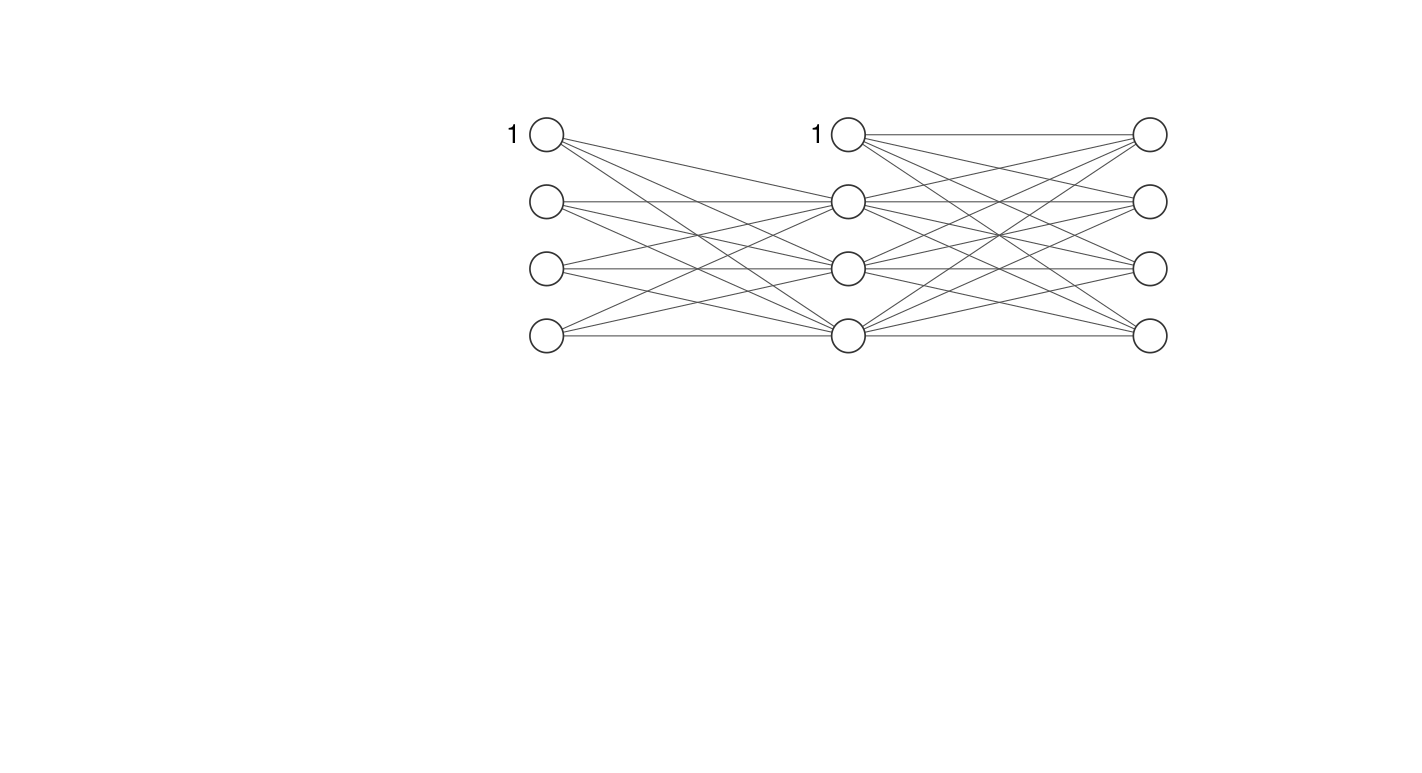
\includegraphics[width=0.8 \textwidth]{nn.png}
	      \end{figure}

	\item Normalizing the training vectors gives us the following normalized dataset.

	      \begin{align*}
		      x_1 = \begin{bmatrix}1 \\ \frac{1}{4} \\ \frac{1}{4}\end{bmatrix}
		      x_2 = \begin{bmatrix}1 \\ \frac{1}{4} \\ 0\end{bmatrix}
		      x_3 = \begin{bmatrix}\frac{1}{2} \\ 0 \\ \frac{1}{4}\end{bmatrix}
		      x_4 = \begin{bmatrix}\frac{1}{2} \\ 0 \\ 0\end{bmatrix}
	      \end{align*}

	\item
	      Let $\sigma$ be the activation function used in the network. We could compute the consecutive outputs by performing a matrix multiplication and then a matrix addition.

	      \[
		      \bm{y} = \sigma(\bm{\Theta}\bm{x} + \bm{b})
	      \]

	      but it is easier to incorporate the bias to our weight matrix, and prepend a unit component to each of our training vectors, as this allows us to perform a single matrix multiplication. In the following, this augmented weight matrix will be denoted $\bm{\Theta}$. The first column of $\bm{\Theta}$ corresponds to the bias weights, and the remaining columns to the given $\bm{\theta}$ values. The normalized training vectors are prepended with a unit row, corresponding to the bias component. We denote an augmented vector with the hat notation $\bm{x} \rightarrow \bm{\hat x}$.

	      We first compute the output at the first hidden layer.

	      \begin{align*}
		      \bm{y}_1^{(1)}
		       & = \sigma\left(\bm{\Theta}^{(1)}\bm{\hat x}_1\right) \\
		       & = \sigma
		      \left(
		      \begin{bmatrix}
				      0.5  & 0    & -0.5 & 0.5 \\
				      -0.5 & 0.5  & -0.5 & 0   \\
				      0.5  & -0.5 & 0    & 0.5 \\
			      \end{bmatrix}
		      \begin{bmatrix}
				      1 \\ 1 \\ 0.25 \\ 0.25
			      \end{bmatrix}
		      \right)                                                \\
		       & = \sigma
		      \left(
		      \begin{bmatrix}
				      0.5 \\ -0.125 \\ 0.125
			      \end{bmatrix}
		      \right)                                                \\
		       & =
		      \begin{bmatrix}
			      0.378 \\ 0.531 \\ 0.469
		      \end{bmatrix}
	      \end{align*}

	      We then use this result to compute the output at the output layer.

	      \begin{align*}
		      \bm{y}_1^{(2)}
		       & = \sigma\left(\bm{\Theta}^{(2)}\bm{\hat y}_1^{(1)}\right) \\
		       & = \sigma
		      \left(
		      \begin{bmatrix}
				      -0.5 & 0.5  & -0.5 & 0.5  \\
				      0.5  & 0    & -0.5 & 0.5  \\
				      -0.5 & -0.5 & 0.5  & 0    \\
				      0.5  & 0.5  & 0    & -0.5 \\
			      \end{bmatrix}
		      \begin{bmatrix}
				      1 \\ 0.378 \\ 0.531 \\ 0.469
			      \end{bmatrix}
		      \right)                                                      \\
		       & = \sigma
		      \left(
		      \begin{bmatrix}
				      -0.342 \\ 0.469 \\ -0.423 \\ 0.454
			      \end{bmatrix}
		      \right)                                                      \\
		       & =
		      \begin{bmatrix}
			      0.585 \\ 0.385 \\ 0.604 \\ 0.388
		      \end{bmatrix}
	      \end{align*}

	      We can now compute the loss for this training sample.

	      \begin{align*}
		      J(\bm{\theta})
		       & = \frac{1}{2} \left\Vert\bm{y}_1^{(2)} - \bm{y}_1\right\Vert^2 \\
		       & = \frac{1}{2}
		      \left\Vert
		      \begin{bmatrix}
			      -0.415 \\ 0.385 \\ 0.604 \\ 0.388
		      \end{bmatrix}
		      \right\Vert^2                                                     \\
		       & = 0.418
	      \end{align*}

	\item We now use the backpropagation algorithm to update the weights matrices, using a learning rate of $\mu = 1$.
	      For the following computations, we will need the derivative of the activation function.

	      \begin{align*}
		      \sigma(u) = \frac{1}{1+e^u} \implies \sigma'(u) = - \frac{e^u}{\left(1+e^u\right)^2} = \sigma(u)(\sigma(u)-1)
	      \end{align*}

	      We start by computing the gradients for both layers.

	      \begin{align*}
		      \delta^{(2)}
		       & = \left(\bm{y}_1^{(2)} - \bm{y}_1\right) \circ \sigma' \left(\bm{\Theta}^{(2)}\bm{y_1^{(1)}}\right) \\
		       & =
		      \begin{bmatrix}
			      -0.415 \\ 0.385 \\ 0.604 \\ 0.388
		      \end{bmatrix} \circ
		      \sigma'
		      \left(
		      \begin{bmatrix}
				      -0.342 \\ 0.469 \\ -0.423 \\ 0.454
			      \end{bmatrix}
		      \right)                                                                                                \\
		       & =
		      \begin{bmatrix}
			      -0.415 \\ 0.385 \\ 0.604 \\ 0.388
		      \end{bmatrix} \circ
		      \begin{bmatrix}
			      -0.243 \\ -0.237 \\ -0.239 \\ -0.238
		      \end{bmatrix}                                                                             \\
		       & =
		      \begin{bmatrix}
			      0.100 \\ -0.091 \\ -0.144 \\ -0.092
		      \end{bmatrix}
	      \end{align*}

	      \begin{align*}
		      \delta^{(1)}
		       & = \bm{\Theta}^{(2)} \delta^{(2)} \circ \sigma' \left(\bm{\Theta}^{(1)} \bm{x_1} \right) \\
		       & =
		      \begin{bmatrix}
			      -0.5 & 0.5  & -0.5 & 0.5  \\
			      0.5  & 0    & -0.5 & 0.5  \\
			      -0.5 & -0.5 & 0.5  & 0    \\
			      0.5  & 0.5  & 0    & -0.5 \\
		      \end{bmatrix}
		      \begin{bmatrix}
			      0.100 \\ -0.091 \\ -0.144 \\ -0.092
		      \end{bmatrix}
		      \circ
		      \sigma'\left(
		      \begin{bmatrix}
				      0.5  & 0    & -0.5 & 0.5 \\
				      -0.5 & 0.5  & -0.5 & 0   \\
				      0.5  & -0.5 & 0    & 0.5 \\
			      \end{bmatrix}
		      \begin{bmatrix}
				      1 \\ 1 \\ 0.25 \\ 0.25
			      \end{bmatrix}
		      \right)                                                                                    \\
		       & =
		      \begin{bmatrix}
			      -0.070 \\
			      0.077  \\
			      -0.077 \\
			      0.051  \\
		      \end{bmatrix}
		      \circ
		      \begin{bmatrix}
			      -0.235 \\
			      -0.249 \\
			      -0.249 \\
		      \end{bmatrix}                                                                 \\
	      \end{align*}

	      As we can see, the dimensions do not seem to match for taking the Hadamard product between $\bm{\Theta}^{(2)} \delta^{(2)}$ and $\sigma' \left(\bm{\Theta}^{(1)} \bm{x_1} \right)$. That's because the gradient of the bias unit does not get backpropagated, as shown in the network structure graph. Therefore, we should not consider the first component of $\bm{\Theta}^{(2)} \delta^{(2)}$.

	      \begin{align*}
		      \delta^{(1)}
		       & =
		      \begin{bmatrix}
			      0.077  \\
			      -0.077 \\
			      0.051  \\
		      \end{bmatrix}
		      \circ
		      \begin{bmatrix}
			      -0.235 \\
			      -0.249 \\
			      -0.249 \\
		      \end{bmatrix} \\
		       & =
		      \begin{bmatrix}
			      -0.018 \\
			      0.019  \\
			      -0.013 \\
		      \end{bmatrix}
	      \end{align*}

	      We now use the gradients to compute the weights update for each layer.

	      \begin{align*}
		      \Delta\bm{\Theta}^{(2)}
		       & = - \mu \delta^{(2)} \bm{y}_1^{(1)T} \\
		       & = -
		      \begin{bmatrix}
			      0.100 \\ -0.091 \\ -0.144 \\ -0.092
		      \end{bmatrix}
		      \begin{bmatrix}
			      1 & 0.378 & 0.531 & 0.469
		      \end{bmatrix}              \\
		       & =
		      \begin{bmatrix}
			      -0.101 & -0.038 & -0.054 & -0.047 \\
			      0.091  & 0.034  & 0.048  & 0.043  \\
			      0.144  & 0.055  & 0.077  & 0.068  \\
			      0.092  & 0.035  & 0.049  & 0.043  \\
		      \end{bmatrix}
	      \end{align*}

	      \begin{align*}
		      \Delta\bm{\Theta}^{(1)}
		       & = - \mu \delta^{(1)} \bm{x}_1^{(1)T} \\
		       & = -
		      \begin{bmatrix}
			      -0.018 \\
			      0.019  \\
			      -0.013 \\
		      \end{bmatrix}
		      \begin{bmatrix}
			      1 & 1 & 0.25 & 0.25
		      \end{bmatrix}              \\
		       & =
		      \begin{bmatrix}
			      0.018  & 0.018  & 0.004  & 0.004  \\
			      -0.019 & -0.019 & -0.005 & -0.005 \\
			      0.013  & 0.013  & 0.003  & 0.003  \\
		      \end{bmatrix}
	      \end{align*}

	      Finally, we update the weights matrices.

	      \begin{align*}
		      \bm{\Theta}^{(2)} & = \bm{\Theta}^{(2)} + \Delta\bm{\Theta}^{(2)} \\
		                        & =
		      \begin{bmatrix}
			      -0.601 & 0.462  & -0.554 & 0.453  \\
			      0.591  & 0.034  & -0.452 & 0.543  \\
			      -0.356 & -0.445 & 0.577  & 0.068  \\
			      0.592  & 0.535  & 0.049  & -0.457 \\
		      \end{bmatrix}
	      \end{align*}

	      \begin{align*}
		      \bm{\Theta}^{(1)} & = \bm{\Theta}^{(1)} + \Delta\bm{\Theta}^{(1)} \\
		                        & =
		      \begin{bmatrix}
			      0.518  & 0.018  & -0.496 & 0.504  \\
			      -0.519 & 0.481  & -0.505 & -0.005 \\
			      0.513  & -0.487 & 0.003  & 0.503  \\
		      \end{bmatrix}
	      \end{align*}
\end{enumerate}
\end{document}
